% ==========================================================================
% LMA Individual Project -- consolidated final report (Phases 1-3)
%
% Build (LuaLaTeX is required: it shapes Devanagari through HarfBuzz):
%   python -m common.report.final --lang hi=Hindi --lang ne=Nepali \
%       --out report/final/tables
%   cd report/final && lualatex report.tex && lualatex report.tex
%
% Hard limit: 10 pages including references. Check with
%   pdfinfo report.pdf | grep Pages
%
% Every table under tables/ is generated from the committed run outputs by
% common/report/final.py -- edit the script, not the .tex files, to change one.
% ==========================================================================
\documentclass[10pt,a4paper]{article}

\usepackage[a4paper,margin=1.8cm]{geometry}
\usepackage[english]{babel}
% Any Devanagari character switches to the Devanagari font automatically, so
% Hindi and Nepali text can be typed directly, in prose and in tables.
\babelprovide[import, onchar=ids fonts]{hindi}
\babelfont{rm}{TeX Gyre Termes}
\babelfont{sf}{TeX Gyre Heros}
\babelfont{tt}{Latin Modern Mono}
\babelfont[hindi]{rm}[Renderer=HarfBuzz,Scale=0.92]{Noto Serif Devanagari}
\babelfont[hindi]{sf}[Renderer=HarfBuzz,Scale=0.92]{Noto Sans Devanagari}
\babelfont[hindi]{tt}[Renderer=HarfBuzz,Scale=0.92]{Noto Sans Devanagari}

\usepackage{amsmath,amssymb}
\usepackage{booktabs,tabularx,multicol}
\usepackage{graphicx}
\usepackage[font=small,labelfont=bf,skip=3pt]{caption}
\usepackage{subcaption}
\usepackage{enumitem}
\usepackage{xcolor}
\usepackage{microtype}
\usepackage{placeins}
\usepackage[hidelinks]{hyperref}

\graphicspath{{../figures/}}
\setlength{\parskip}{2pt}
\setlength{\emergencystretch}{2em}
\setlength{\textfloatsep}{8pt plus 2pt minus 2pt}
\setlength{\floatsep}{6pt plus 2pt minus 2pt}
\setlength{\intextsep}{6pt plus 2pt minus 2pt}
\setlist{nosep,leftmargin=*}
\setlength{\tabcolsep}{4pt}
\renewcommand{\topfraction}{0.9}
\renewcommand{\bottomfraction}{0.6}
\renewcommand{\textfraction}{0.1}
\renewcommand{\floatpagefraction}{0.85}
\setcounter{topnumber}{3}
\setcounter{bottomnumber}{2}
\setcounter{totalnumber}{5}

% Draft notes print in red while \drafttrue; switch to \draftfalse before
% submitting and check that nothing marked TODO is left in the text.
\newif\ifdraft
\draftfalse
\newcommand{\todo}[1]{\ifdraft{\color{red}\textbf{[TODO: #1]}}\fi}

\newcommand{\MH}{Model~H}
\newcommand{\ML}{Model~L}
\newcommand{\code}[1]{\texttt{#1}}
\newcommand{\tablefile}[1]{\input{tables/#1.tex}}

\title{\vspace{-1.2cm}\textbf{Building and Analysing Monolingual Transformer Language Models\\in Hindi and Nepali}\\[2pt]
\large Language Models and Agents, Monsoon 2026 --- Individual Project: Final Report}
\author{Saksham Goyal\\\normalsize Roll no.\ 2024115005}
\date{\vspace{-0.6cm}}

\begin{document}
\maketitle

\begin{abstract}
\noindent
Two independent decoder-only Transformers of 24.1M parameters were built and trained from scratch:
\MH{} on 523.7M training tokens of Hindi and \ML{} on 357.5M tokens of Nepali, with separate corpora, tokenizers, vocabularies and weights.
\MH{} reaches lower test perplexity (42.9 against 47.1) but \ML{} reaches lower bits-per-byte (0.448 against 0.557), because the Nepali tokenizer packs more text into each token.
After finetuning on synthetic comparative-reasoning data in each language, both models learn the answer format (exact match rises from 0\%), but they learn the comparison itself only weakly: \MH{} reaches 40.8\% against a 37.8\% chance baseline on held-out names and \ML{} stays at chance.
Error and attention analysis show why. Finetuning taught the models to attend to the entities in the prompt and to follow surface shortcuts, not to decide \emph{which} entity is correct.
\end{abstract}

% ==========================================================================
\section{Introduction}
% ==========================================================================
The project builds the whole pipeline twice, once per language: corpus collection and cleaning, tokenizer training, a hand-written Transformer, pretraining, evaluation, reasoning finetuning and attention analysis.
Hindi is the higher-resource language, with the largest body of openly licensed Devanagari text of any Indian language.
Nepali, from the permitted lower-resource list, was chosen over Maithili and Bhojpuri. It shares the Devanagari script, so one normalisation pipeline serves both models, but it is far enough from Hindi that the two are reliably separable. Maithili and Bhojpuri sit inside the Hindi dialect continuum, and text labelled as either is often Hindi, which would have put the ``no shared data'' constraint at risk.
Only implementation code is shared. All data, tokenizers, checkpoints and run logs live under \code{Hindi/} or \code{Nepali/}.
Every table in this report is generated from committed run outputs by \code{common/report/final.py}.
The per-phase reports (\code{report/phase1.md}, \code{report/phase2.md}) hold the full tables this report condenses.

% ==========================================================================
\section{Data and tokenizers (Phase 1)}
% ==========================================================================
\subsection{Corpora}
Each corpus combines two downloaded sources, the verified split of Sangraha~\cite{sangraha} and CC-100~\cite{ccnet}, with manually collected text (Table~\ref{tab:corpus}).
For Hindi, the manual part comes from Wikimedia dumps (mainly Wikisource's proofread public-domain literature and Wikipedia) and three news sites fetched with my own crawler.
For Nepali, it comes from three Wikimedia dumps and 18 news sites.
Crawling honours \code{robots.txt} and each site's crawl delay, and raw bytes are stored so that extraction can be re-run without re-fetching.
Manual collection is 29.5\% (Hindi) and 22.9\% (Nepali) of training tokens. Both shares are measured on tokens \emph{after} deduplication and clear the 20\% floor.

\begin{table}[t]
\centering\small
\begin{minipage}[b]{0.66\linewidth}\centering
\tablefile{corpus}
\caption{Corpus statistics. Tokens are counted by encoding every document with the chosen 16k tokenizer.}
\label{tab:corpus}
\end{minipage}\\[6pt]
\begin{minipage}[b]{0.62\linewidth}\centering
\tablefile{tokenizer}
\caption{Tokenizer sweep on 2{,}000 held-out validation documents. Fertility is tokens per whitespace word; byte fallback is the share of tokens that are raw bytes. The unknown-token rate is zero at every size (see text).}
\label{tab:tokenizer}
\end{minipage}
\end{table}

\subsection{Cleaning pipeline}
Both languages run the same code on separate data (\code{common/pipeline/}):
\begin{enumerate}
\item \textbf{Normalisation.} Text is converted to Unicode NFC and zero-width joiners are removed. A \emph{matra repair} table rewrites legacy two-codepoint vowel signs (for example \textsc{aa}+\textsc{e} for \textsc{o}). NFC does not fix these, because U+094B has no canonical decomposition. Left alone, the frequent Nepali suffix को would be split into two unrelated token sequences.
\item \textbf{Quality filters} with a recorded reason: length bounds, a minimum of 60\% Devanagari letters, digit and punctuation ratio caps, and a repeated-line check that catches listing pages.
\item \textbf{Deduplication.} Exact duplicates are found by SHA-256. Near-duplicates are found with MinHash (128 permutations over 5-word shingles) and LSH (16 bands of 8, a similarity threshold near 0.76), with clusters merged by union-find. When a cluster collapses, the \emph{manually collected} copy is kept. CC-100 is built from Common Crawl, which crawled Wikipedia, so otherwise dedup would silently move documents from manual to downloaded and erode the manual share.
\item \textbf{Splits} are assigned per document from a salted SHA-256 of its id (about 98/1/1), so no article spans two splits, and adding a source never moves an existing document.
\end{enumerate}

\subsection{Tokenizers}
Each language has a SentencePiece unigram tokenizer~\cite{sentencepiece,unigram} trained on its own training split only.
\code{byte\_fallback} is on, so an unseen character becomes UTF-8 bytes rather than \code{<unk>}. The unknown rate is therefore zero by construction, and the byte-fallback rate is the meaningful diagnostic.
The vocabulary size was chosen from a sweep (Table~\ref{tab:tokenizer}).
Fertility falls monotonically with vocabulary size, so it cannot choose a size on its own.
Two things argue against the largest vocabulary. First, vocabulary utilisation drops from about 97\% to 91\% (Hindi) and 89\% (Nepali) at 32k, and rarely seen entries get poorly trained embeddings. Second, a 32k vocabulary at $d=384$ costs 12.3M parameters, half of the 25M budget.
Both sweeps independently select 16{,}000.

\subsection{The Nepali shortfall}
\ML{} has 357.5M training tokens, 0.71$\times$ the 500M target. The limit is not the supply of Nepali text: Sangraha alone holds more, and several hundred thousand discovered news articles were never fetched.
The limit is the manual floor. A corpus can be at most five times its manual part, and manual collection is bounded by polite crawl rates (about one request per second per host).
Nepali was trained for one epoch rather than repeated to reach 500M, so the two models see different amounts of data. Section~\ref{sec:discussion} returns to what that does to the comparison.

% ==========================================================================
\section{Model and pretraining (Phase 2)}
% ==========================================================================
\subsection{Architecture}
Both models share the same geometry, so the comparison is between languages and corpora, not architectures. Weights, data and vocabularies remain separate.
Each is a GPT-style decoder~\cite{vaswani,gpt2} built only from \code{nn.Linear}, \code{nn.Embedding}, \code{nn.LayerNorm} and \code{nn.Dropout}, with 10 layers, $d=384$, 6 heads ($d_k=64$), a GELU feed-forward of width 1536, a context of 512, and dropout 0.1.
Pre-norm blocks~\cite{prenorm} keep an un-normalised residual path from input to output, so gradients reach early layers undistorted.
Positions are \emph{learned absolute} embeddings. They cost one $512\times384$ table, but they make 512 a hard limit, since no position beyond it has a representation.
The output head is tied to the token embedding~\cite{tying}, which saves $16{,}000\times384=6.1$M parameters, a quarter of the budget.
The total is \textbf{24,086,016} parameters: embedding 6,144,000, positions 196,608, blocks 17,744,640, final LayerNorm 768.

In attention, heads are carved from the \emph{feature} axis. $(B,T,d)$ is viewed as $(B,T,h,d_k)$ and only then transposed to $(B,h,T,d_k)$.
Viewing directly to $(B,h,T,d_k)$ would slice along \emph{time}. That bug still trains and still gives a falling loss curve.
Scaling by $1/\sqrt{d_k}$ keeps the variance of $q\cdot k$ near one. Without it, the standard deviation would be $\sqrt{64}=8$, the softmax would saturate at initialisation, and its gradient would vanish.
The causal mask is additive ($0$ or $-\infty$) and applied \emph{before} the softmax, so future positions receive exactly zero weight and each row still sums to one.

\subsection{Verifying the implementation}
A falling loss curve does not show that attention is correct, so correctness is asserted in \code{tests/}:
(i)~changing token $t{+}1$ leaves the logits at $t$ \emph{bitwise} identical;
(ii)~no gradient path runs from later positions to output~$t$;
(iii)~the batched head reshape matches a reference that splits heads by explicit column slicing;
(iv)~attention rows sum to one and have an exactly zero upper triangle;
(v)~loss at initialisation is $\ln 16000 = 9.68$;
(vi)~resuming from a checkpoint reproduces an uninterrupted run's losses \emph{exactly}.
Checkpoints hold weights, AdamW moments, the schedule, the fp16 loss scale, the step, the data position and the RNG state, and batches are a pure function of (seed, step).

\subsection{Pretraining}
Training used AdamW~\cite{adamw} ($\beta=(0.9,0.95)$, weight decay 0.1 on matrices only), a 6e-4 peak learning rate with 1.5\% warmup and cosine decay to 6e-5, 32,768 tokens per step (micro-batch 16 $\times$ accumulation 4 $\times$ 512), gradient clipping at 1.0, and fp16 on a Kaggle T4 (Table~\ref{tab:pretraining}, Fig.~\ref{fig:loss}).
Each model saw exactly one epoch of its own corpus.

\begin{figure}[t]
\centering
\begin{minipage}[b]{0.46\linewidth}\centering\footnotesize
\tablefile{pretraining}
\captionof{table}{Pretraining runs. The packed arrays hold one EOS token per document on top of the Phase~1 counts.}
\label{tab:pretraining}
\end{minipage}\hfill
\begin{minipage}[b]{0.50\linewidth}\centering
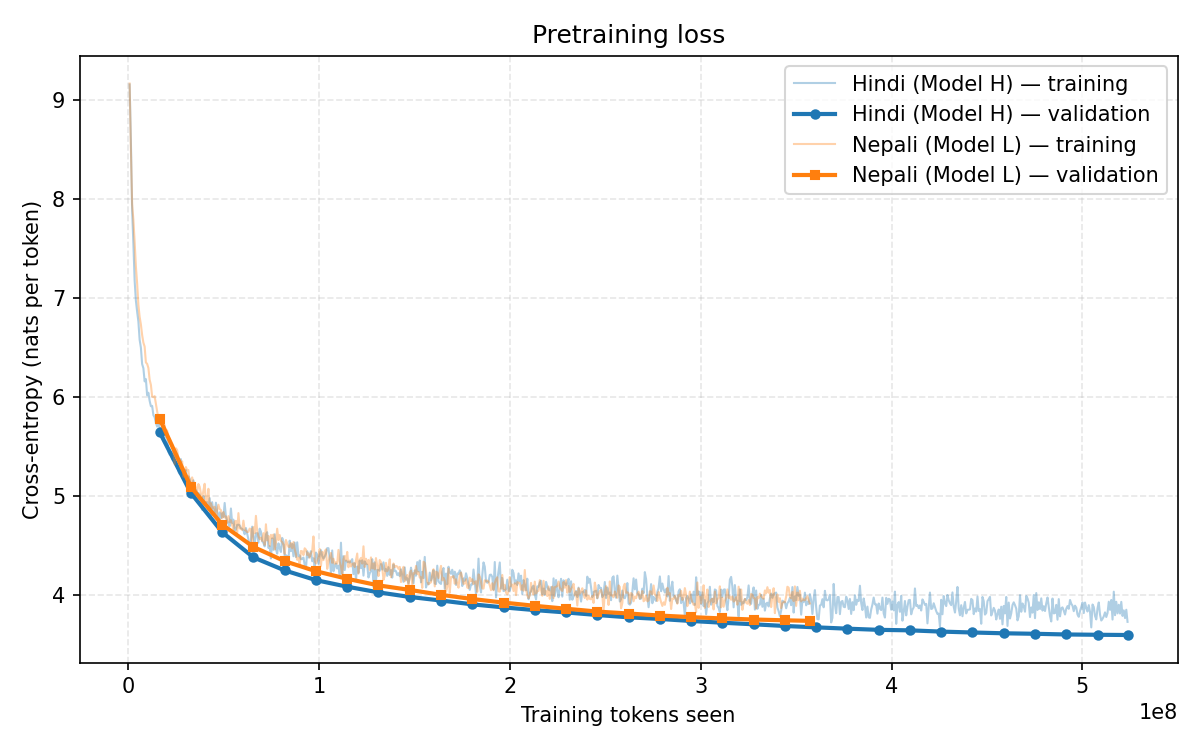
\includegraphics[width=\linewidth]{pretraining_loss_by_tokens.png}
\caption{Training and validation loss against tokens seen.}
\label{fig:loss}
\end{minipage}
\end{figure}

% ==========================================================================
\section{Language-model evaluation (Phase 2)}
% ==========================================================================
\subsection{Perplexity and bits-per-byte}
\begin{table}[t]
\centering\small
\tablefile{lm}
\caption{Held-out language modelling. CE is in nats per token and BPB in bits per UTF-8 byte. Each model is scored on its own complete split.}
\label{tab:lm}
\end{table}

\MH{} has the lower perplexity, but \ML{} has the lower bits-per-byte (Table~\ref{tab:lm}), and the disagreement has a measurable cause.
Perplexity is per token, and the two tokenizers are independent, so a token is not the same amount of text in the two models.
A Nepali token carries 12.40 bytes against 9.74, 27\% more, while its cross-entropy is only 2.5\% higher. Dividing the same likelihood by bytes instead of tokens reverses the ranking.
This is \emph{not} evidence that \ML{} is the better model, because the two are scored on different text.
It does show that the obvious reading of the perplexity column, that the lower-resource model is clearly worse, is an artefact of tokenizer granularity.
Both corpora are Devanagari, which UTF-8 encodes in three bytes per character, so these BPB values are low in absolute terms and should not be compared with published figures for English.

\subsection{Generation}
Continuations of about 70 tokens for held-out test prefixes (59 Hindi and 50 Nepali prompts) were scored against the true continuation (Table~\ref{tab:generation}).
The overlap metrics~\cite{bleu,chrf,rouge,sacrebleu} are weak evidence for open-ended generation, since a prompt has many valid continuations and the test set contains only one.
BLEU-4 is close to all-or-nothing per word, because Hindi and Nepali attach case markers to stems.
chrF matches character $n$-grams, so a correct stem with the wrong suffix earns partial credit, which makes it the most informative of the three here.
ROUGE-L is computed by our own implementation, because the \code{rouge-score} tokenizer deletes every non-ASCII character and scores every Devanagari pair as zero.
Greedy decoding degenerates into loops in both models (4-gram repetition of 0.78 and 0.75)~\cite{degeneration}, which is also why BLEU peaks under greedy decoding while chrF does not.
At $T{=}1.0$ the text is well-formed: postpositions attach correctly, verb endings agree, and sentences end with a danda. But coherence lasts only about a sentence, and numbers and facts are confabulated.
The failure modes of the two models are the same in kind and close in degree.

\begin{table}[t]
\centering\small
\begin{minipage}[t]{0.55\linewidth}\centering\vspace{0pt}\footnotesize
\tablefile{generation}
\caption{Generation quality. Rep-4 is the share of repeated 4-grams; Dist-$n$ is the share of unique $n$-grams.}
\label{tab:generation}
\end{minipage}\hfill
\begin{minipage}[t]{0.42\linewidth}\centering\vspace{0pt}
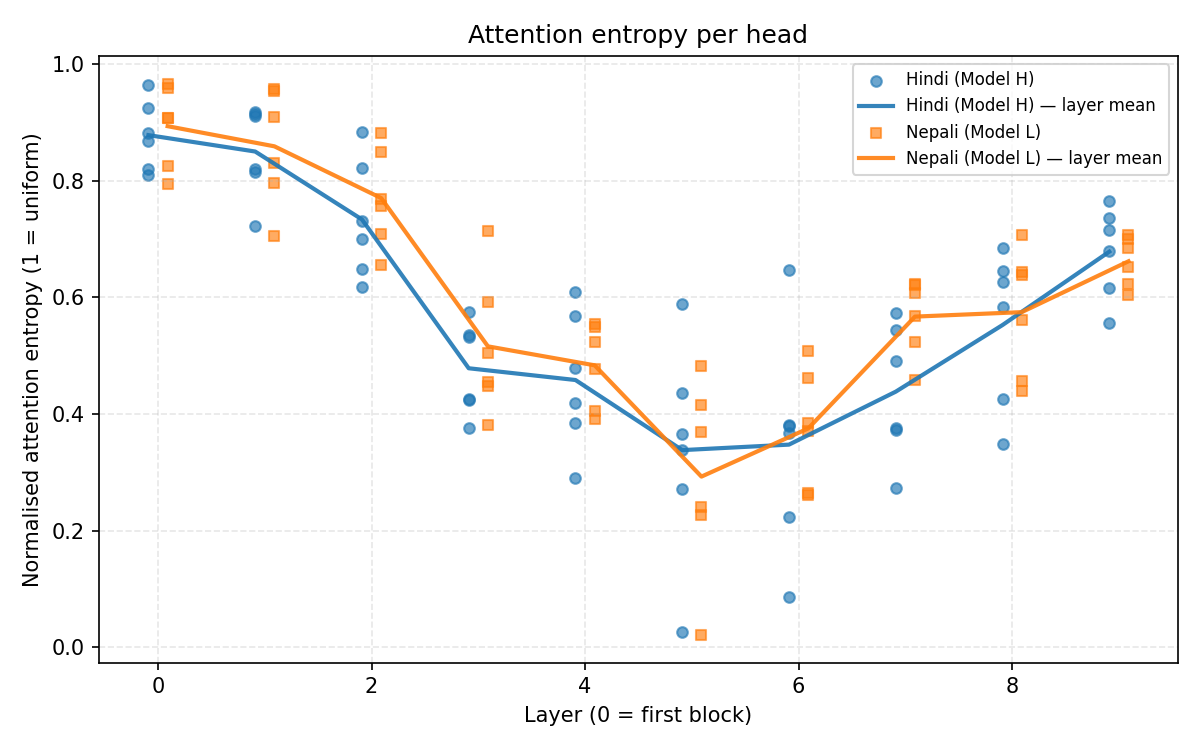
\includegraphics[width=\linewidth]{attention_entropy.png}
\captionof{figure}{Normalised attention entropy for every head (dots) and the layer mean (lines), on held-out corpus text.}
\label{fig:entropy}
\end{minipage}
\end{table}

\subsection{Attention}
Every head's normalised entropy (entropy divided by $\log(i{+}1)$) and mean attention distance were measured on 32 held-out windows (Table~\ref{tab:heads}, Fig.~\ref{fig:entropy}).
The two models, trained independently on different corpora, organised their heads the same way:
diffuse, long-range layers 0--2 (normalised entropy 0.73--0.89);
a sharp, local middle band that contains a \emph{previous-token head} in layer~5 of each model (entropy about 0.02, distance 1.2; Fig.~\ref{fig:heatmap});
and late layers that widen again into content-dependent attention.
Some heads are sharp but have a mean distance above 100 positions. They put nearly all their mass on position~0, the attention-sink pattern~\cite{sinks}.
The difference between the resource tiers is in \emph{specialisation}. \MH{} has 16 sharp heads to \ML{}'s 10.
In the last four layers, the spread of head distances within a layer averages 125 positions for \MH{} against 61 for \ML{}: the late heads of the lower-resource model behave more alike.

\begin{table}[t]
\centering\small
\tablefile{heads}
\caption{Head types among the 60 heads of each model. Local: mean distance $<5$. Sharp: normalised entropy $<0.4$. Diffuse: $>0.7$. Sink-like: sharp and distance $>100$.}
\label{tab:heads}
\end{table}

\begin{figure}[t]
\centering
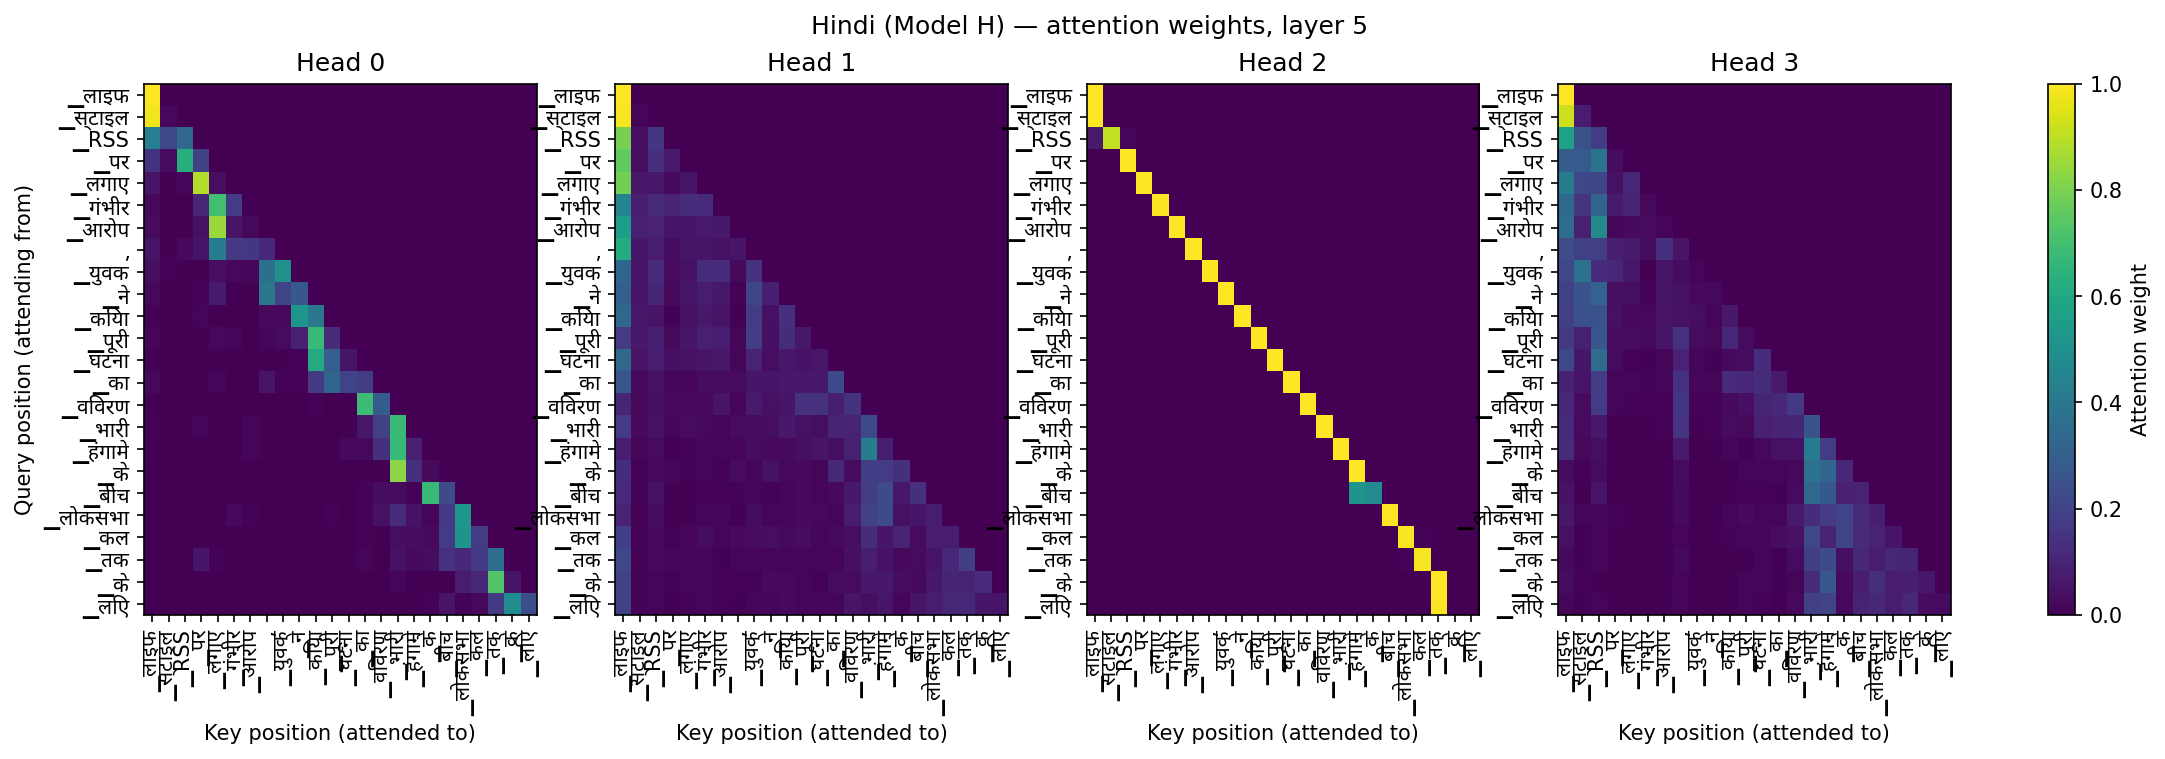
\includegraphics[width=0.9\linewidth]{attention_heatmap_hindi_layer5.png}
\caption{\MH{}, layer 5, on held-out text. Head 2 is a previous-token head. Every map is lower-triangular, which is the causal mask directly visible. (Axis labels are drawn by matplotlib, which does not shape Devanagari, so some vowel signs look detached.)}
\label{fig:heatmap}
\end{figure}

\FloatBarrier
% ==========================================================================
\section{Reasoning finetuning (Phase 3)}
% ==========================================================================
\subsection{Synthetic dataset}
The generator (\code{common/\allowbreak reasoning/\allowbreak generate.py}) fills templates from each language's own lexicon (\code{configs/\allowbreak reasoning.yaml}), so every label is known by construction.
There are four task families in equal proportion over four attributes (height, age, weight, price):
\textbf{numeric pair}, two stated values, asking which is greater or smaller or whether they are equal (a fifth of pairs are tied, so ``both equal'' is a real answer);
\textbf{numeric triple}, asking for the largest or smallest of three values;
\textbf{chain superlative}, with only pairwise statements such as ``A is taller than B'' in shuffled order and randomly phrased with the greater or smaller adjective, asking for the extreme;
and \textbf{chain relation}, a yes/no question about two entities that, four times in five, are never compared directly.
The templates follow each language's own grammar rather than a translation of one into the other.
Hindi adjectives agree with the subject's gender (लंबा/लंबी).
Nepali attaches the comparative postposition to the name (सुनिताभन्दा जेठो छ) and changes the copula for a feminine subject (छ/छिन्).
Numbers are written in the digits each corpus mostly uses: ASCII for Hindi and Devanagari for Nepali.

\textbf{Leakage.} Entity names are partitioned 60/20/20 into train, validation and test pools \emph{before} any example is generated (Table~\ref{tab:rdata}). A test question can therefore only be answered by comparing, not by recalling facts about a name.
The run's \code{dataset\_stats.json} records zero name overlap between splits and zero duplicated prompts, and a test (\code{tests/\allowbreak test\_reasoning\_data.py}) re-derives every label from the prompt text.
A fourth split, \code{test\_long}, uses test names with five-entity chains, one entity longer than anything in training.

\begin{table}[t]
\centering\small
\tablefile{reasoning_data}
\caption{Reasoning datasets. Names are disjoint across train, validation and test. \code{test\_long} reuses the test names with longer chains. Tokens are counted with each language's own tokenizer.}
\label{tab:rdata}
\end{table}

\subsection{Protocol, and how it was reached}
Each model starts from its own pretrained \code{best.pt} (fresh AdamW state, tokenizer unchanged). The loss is cross-entropy on the answer tokens and EOS only, with prompt targets masked.
The final configuration uses an effective batch of 128, 750 steps (4.8 epochs), a 1e-4 peak with 50 warmup steps and cosine decay to 1e-5, weight decay 0.1, clipping at 1.0, dropout 0.1, and a \emph{frozen} tied embedding and output head.
Validation exact match on 512 held-out-name examples is checked every 50 steps, and \code{best.pt} keeps the best one.
Checkpoints use the same resumable format as pretraining. Both runs took about 1.5 hours on a CPU, since sequences are only about 34 tokens long.

The configuration came from the short runs in Table~\ref{tab:ablations}.
The first attempt (\code{v1\_unfrozen\_48names}) had a trainable embedding and only 48 training names.
Its validation loss \emph{rose} while training loss fell. Of 128 held-out questions with an entity answer, 106 were answered with a \emph{training} name that did not appear in the prompt: the finetune had turned the training names into an answer vocabulary.
Freezing the tied embedding removes the direct route to that shortcut, and enlarging the name pools to about 200 people per language weakens it further. After both changes, 187 of 196 entity answers named an entity from the prompt.
At batch 32 and a 3e-4 peak, validation accuracy fell once the learning rate reached its peak. Each example supervises only one or two tokens, so a batch of 32 is only about 50 target tokens, too noisy for a large learning rate. That is what led to batch 128 and a 1e-4 peak.

\begin{table}[t]
\centering\footnotesize
\tablefile{ablations}
\caption{Finetuning runs (validation exact match on held-out names). All start from the same pretrained checkpoint. Runs with \code{48names} used the first, smaller lexicon.}
\label{tab:ablations}
\end{table}

\subsection{Results}
\begin{table}[t]
\centering\small
\tablefile{reasoning_results}
\caption{Accuracy (\%) before and after finetuning. \emph{Exact}: greedy decoding to EOS equals the answer. \emph{Choice}: the candidate with the highest summed log-probability. \emph{Chance}: the mean of $1/|\text{candidates}|$. The pretrained model's exact match is 0.0 everywhere, so only its choice accuracy is shown.}
\label{tab:rresults}
\end{table}

Table~\ref{tab:rresults} shows three results.
\textbf{First, finetuning teaches the format.} Pretrained exact match is 0\%, since neither model ever emits a bare answer followed by EOS. After finetuning, 99\% (H) and 97\% (L) of greedy outputs are one of the candidate answers.
\textbf{Second, the comparison is learned only weakly.}
\MH{} reaches 40.8\% on \code{test} against 37.8\% chance. With $n=2000$ the standard error is about 1.1 points, so that is about 2.7 standard errors above chance.
\ML{} reaches 37.5\% against 37.7\%, which is chance.
Most of \MH{}'s gain comes from chain superlative (16.8$\to$34.4\%) and chain relation (48.0$\to$52.8\%).
\textbf{Third, the resource gap shows up most on longer chains.} On \code{test\_long} with four hops, \MH{} rises above chance (29.5\% against 23.5\%) while \ML{} stays below it (18.3\%).
Validation selection flatters both models: the best validation exact match (46.7\% and 41.0\%, both at step~200) was chosen from 16 noisy evaluations of 512 examples, and the untouched test set is the honest number.

\subsection{Error analysis}
Table~\ref{tab:errors} measures how often answers follow a shortcut rather than the comparison. Table~\ref{tab:examples} gives examples.
\begin{itemize}
\item \textbf{The pretrained model copies repeated names.} In a chain, inner entities appear in two statements and the two ends in one, and the extreme being asked for is always an end.
The pretrained models' preferred candidate is an inner entity 69\% (H) and 60\% (L) of the time, which is consistent with a language model preferring a name it has just seen twice.
This is why pretrained accuracy on chain superlatives (16.8\% and 20.2\%) sits well \emph{below} chance.
Finetuning cuts the inner-entity rate to 26--28\%. Much of the superlative gain is consistent with this shortcut, which needs no transitive reasoning.
\item \textbf{Each finetuned model settles on a default answer.} \MH{} answers ``no'' to 83\% of relation questions (53\% of gold answers are ``no''). \ML{} answers ``both equal'' to 51\% of greater/smaller pair questions, where the gold rate is 22\%, so it rarely compares the two numbers at all.
\item \textbf{Recency.} Both finetuned models over-select the last-mentioned entity (51\% and 45\% against 38--39\% in the gold answers).
\end{itemize}

\begin{table}[t]
\centering\small
\tablefile{errors}
\caption{Shortcuts in the answers on \code{test}. \emph{Pre} is the pretrained model's highest-likelihood candidate (its greedy output is never a candidate), \emph{FT} is the finetuned greedy output, and \emph{Gold} is the rate in the correct answers.}
\label{tab:errors}
\end{table}

\begin{table}[t]
\centering\small
\tablefile{examples}
\caption{The first correct and first incorrect three-entity chain superlative in each model's test predictions (not hand-picked). The Hindi failure returns अतुल, the middle of the chain. The Nepali failure returns सुशील, the youngest, when the question asks for the oldest.}
\label{tab:examples}
\end{table}

% ==========================================================================
\section{Attention after finetuning (Phase 3)}
% ==========================================================================
The Phase~2 statistics were re-run on both checkpoints over 400 reasoning test prompts and over held-out corpus text (Table~\ref{tab:attshift}, Figs.~\ref{fig:ftheat} and~\ref{fig:answerpos}). The analysis also measures where the final prompt token, the position that predicts the answer, sends its attention.
\begin{itemize}
\item \textbf{General attention is almost untouched.} On corpus text, mean entropy and distance change by at most 0.007 and 1.6 positions. The early layers look essentially identical before and after (Fig.~\ref{fig:ftheat}, left). Only 200 steps at a low learning rate, with the embedding frozen, were not enough to overwrite pretraining.
\item \textbf{Local vs.\ long-range attention barely moves.} On reasoning prompts, mean distance changes by $+0.02$ (H) and $+0.59$ (L) positions. There is no general shift from local to long-range attention.
\item \textbf{Changes are spread over many heads, and they differ between models} (Fig.~\ref{fig:answerpos}b). In \MH{}, the largest single change is layer 2, head 2, which became more diffuse by 0.4. In \ML{}, every head in layer~9 became sharper.
\item \textbf{Late layers learned to look at the entities, but not at the right one.} From the answer position, the share of attention on entity names rises from 0.18 to 0.31 (both models), and in layer~9 from 0.54 to 0.66 (H) and from 0.45 to 0.62 (L). The correct entity's \emph{share} of that entity attention hardly changes: 0.32$\to$0.33 across layers, and +2 (H) and +4 (L) points in layer~9.
\end{itemize}
The attention results therefore match the accuracy results. Finetuning taught the models \emph{where} an answer comes from, a name in the prompt, but not how to choose \emph{which} name. That is exactly the behaviour one would expect from a model that has learned the answer format and a few shortcuts, but not the comparison.

\begin{table}[t]
\centering\small
\tablefile{attention_shift}
\caption{Attention before and after finetuning, averaged over heads. Entropy is normalised and distance is in tokens. \emph{Answer pos.\ $\to$ entities} is the attention mass from the final prompt token onto entity-name tokens. \emph{Gold share} is the correct entity's fraction of that mass.}
\label{tab:attshift}
\end{table}

\begin{figure}[t]
\centering
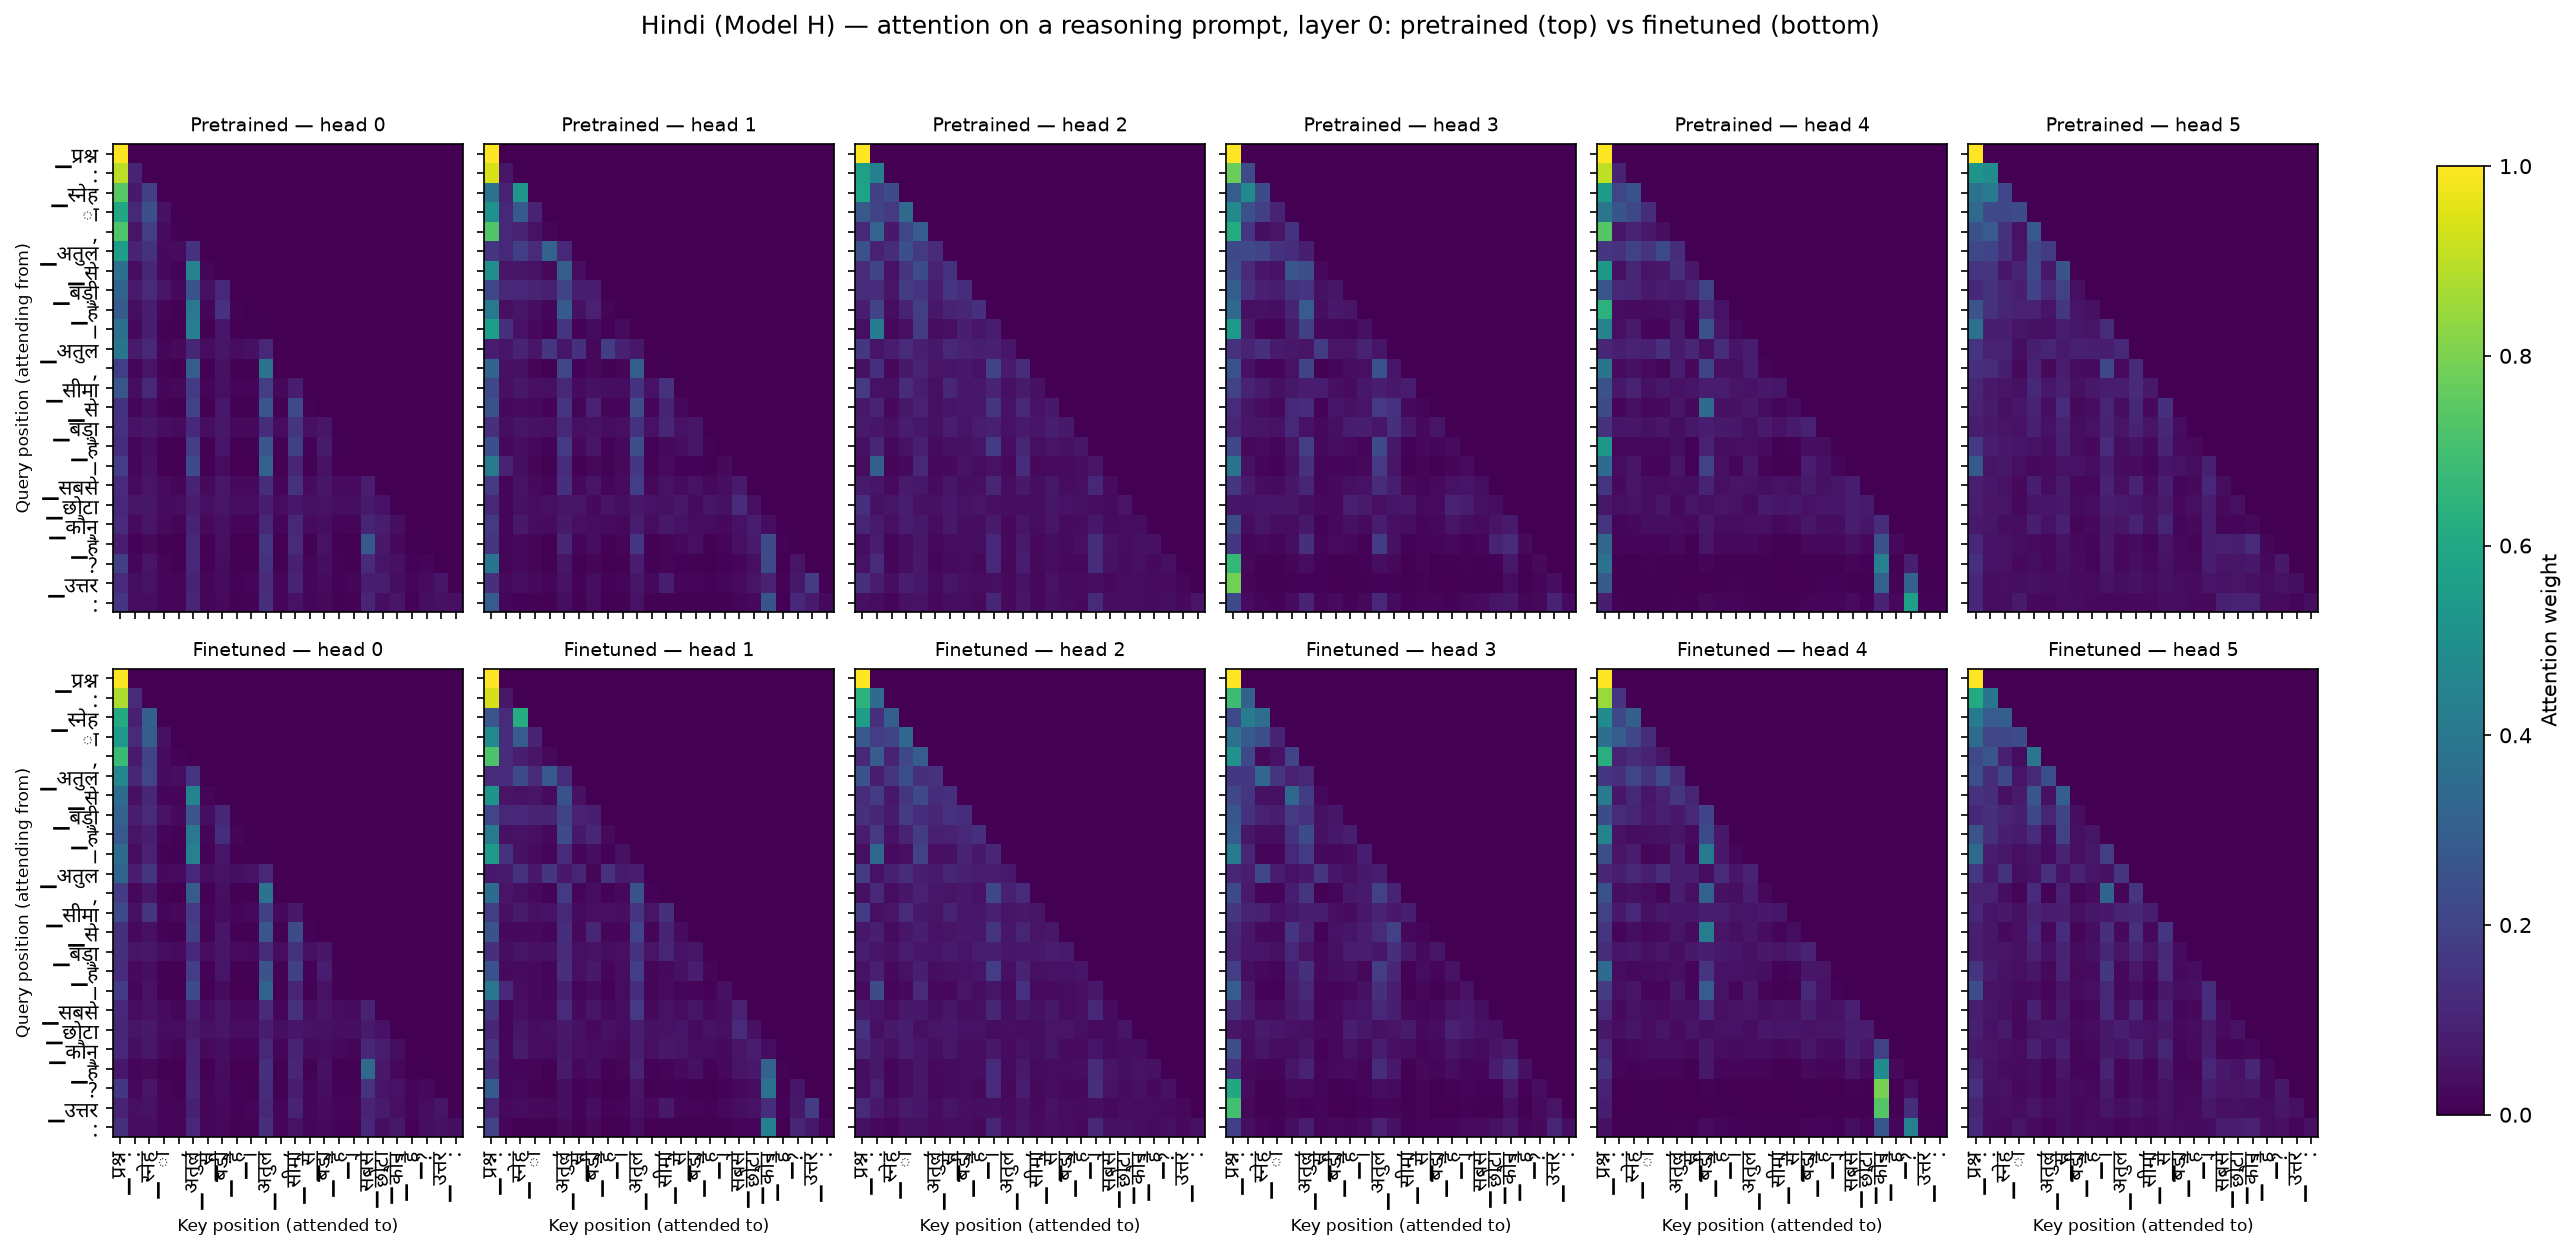
\includegraphics[width=0.495\linewidth]{attention_finetune_hindi_layer0.png}\hfill
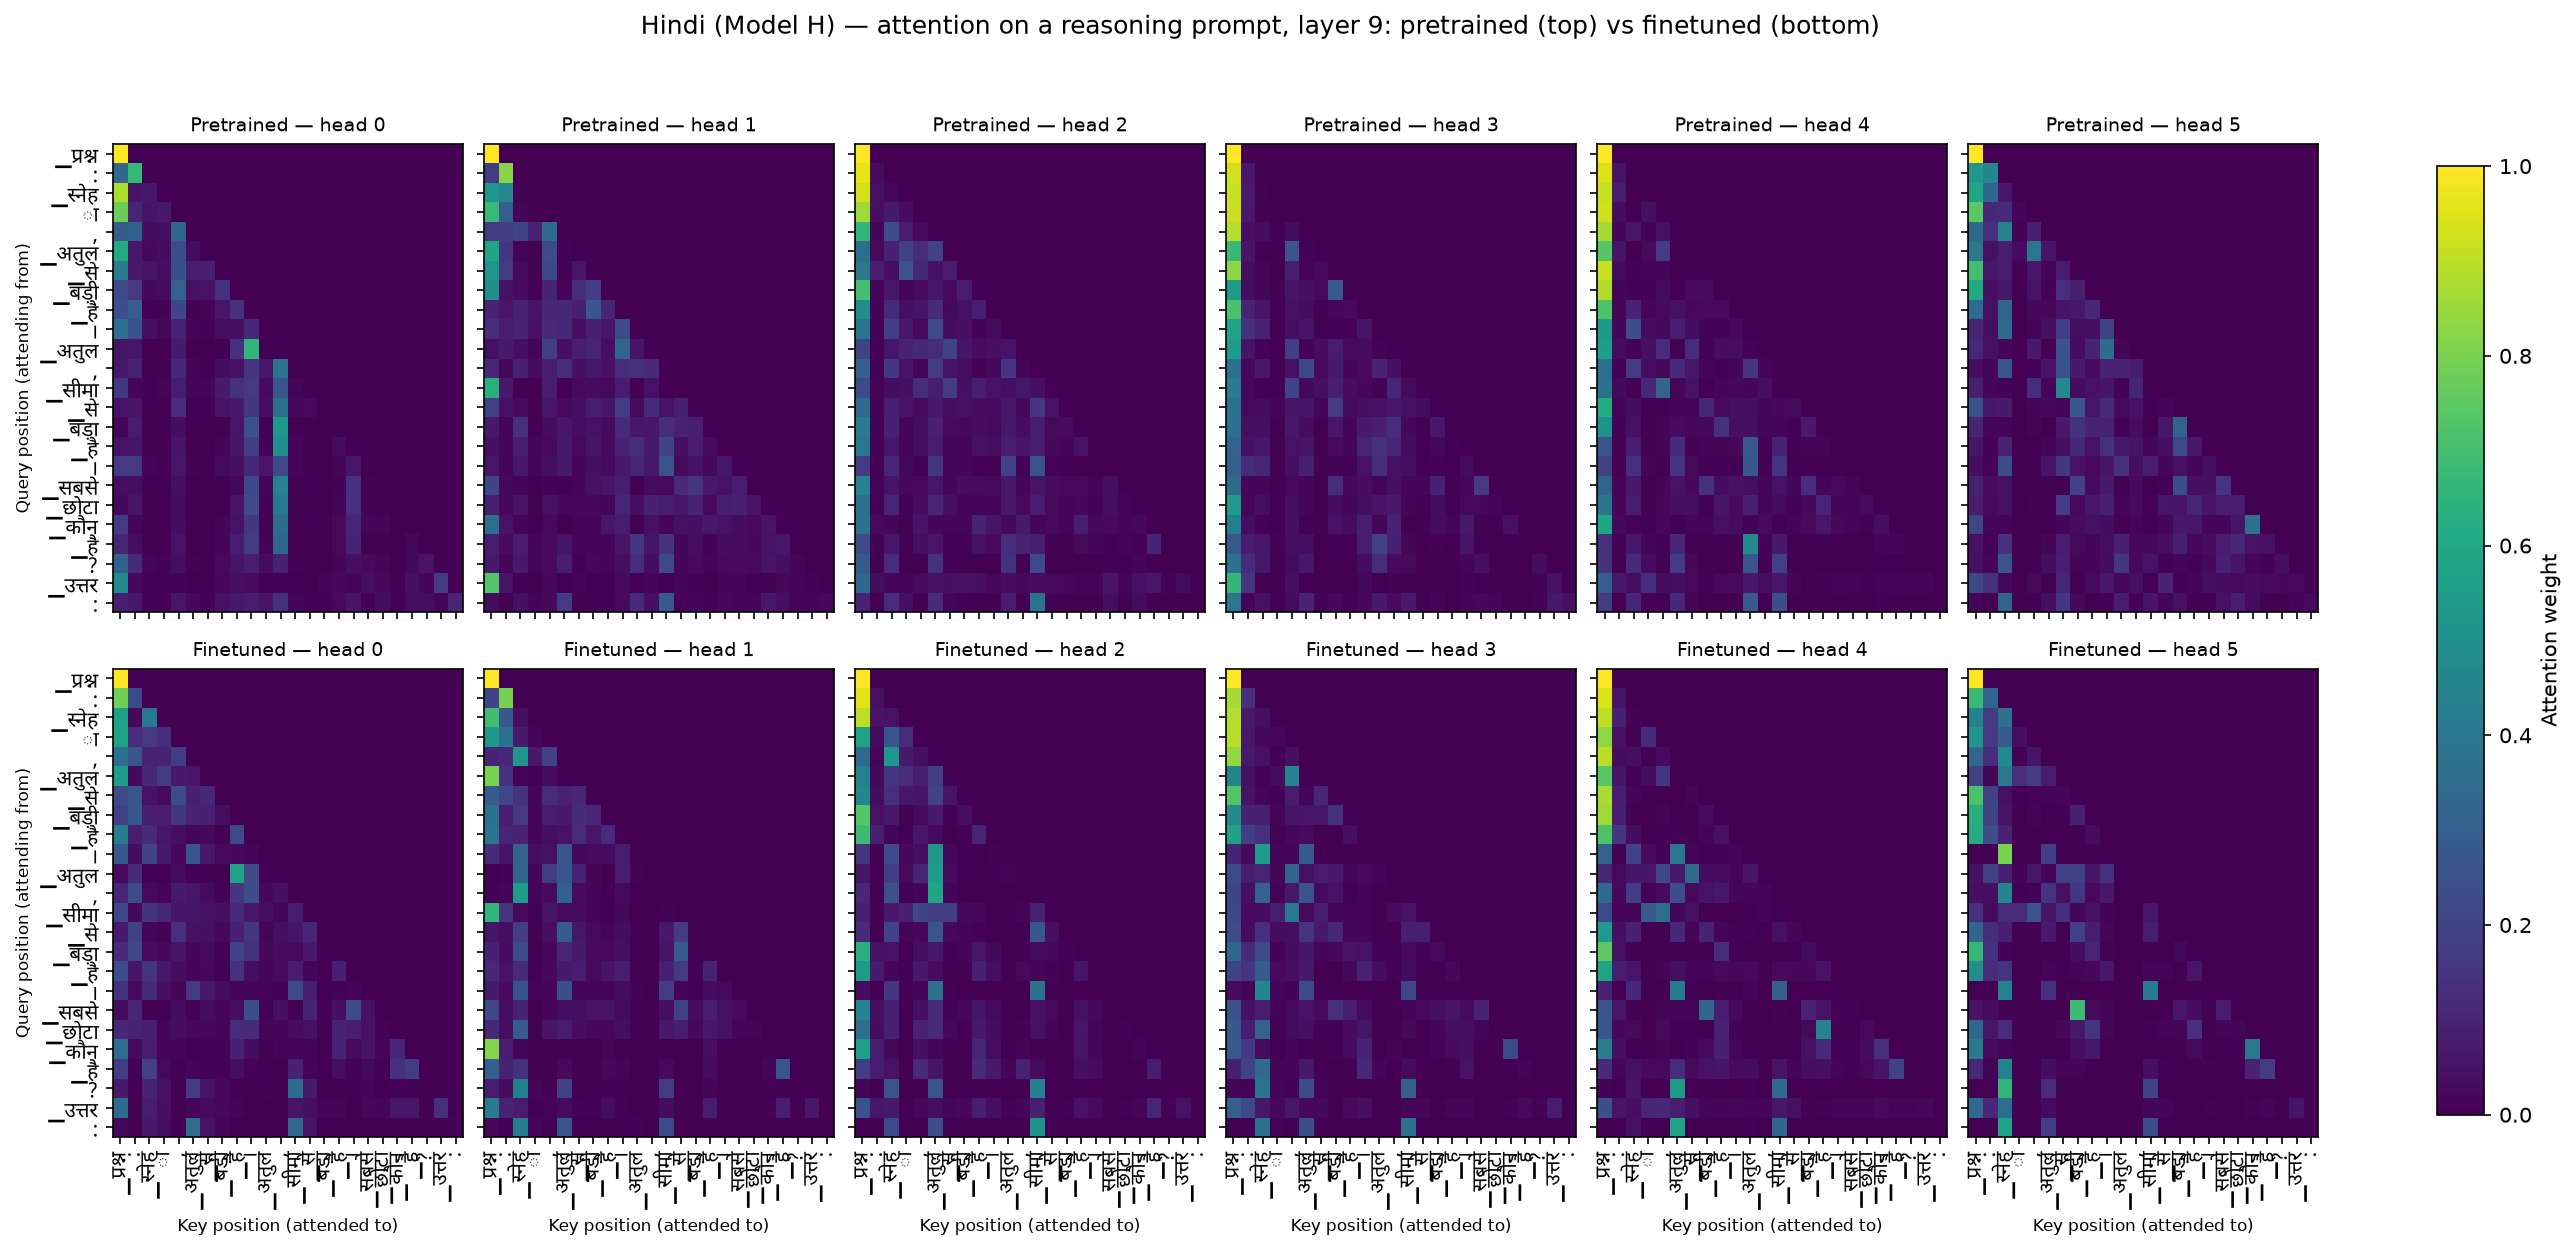
\includegraphics[width=0.495\linewidth]{attention_finetune_hindi_layer9.png}\\[2pt]
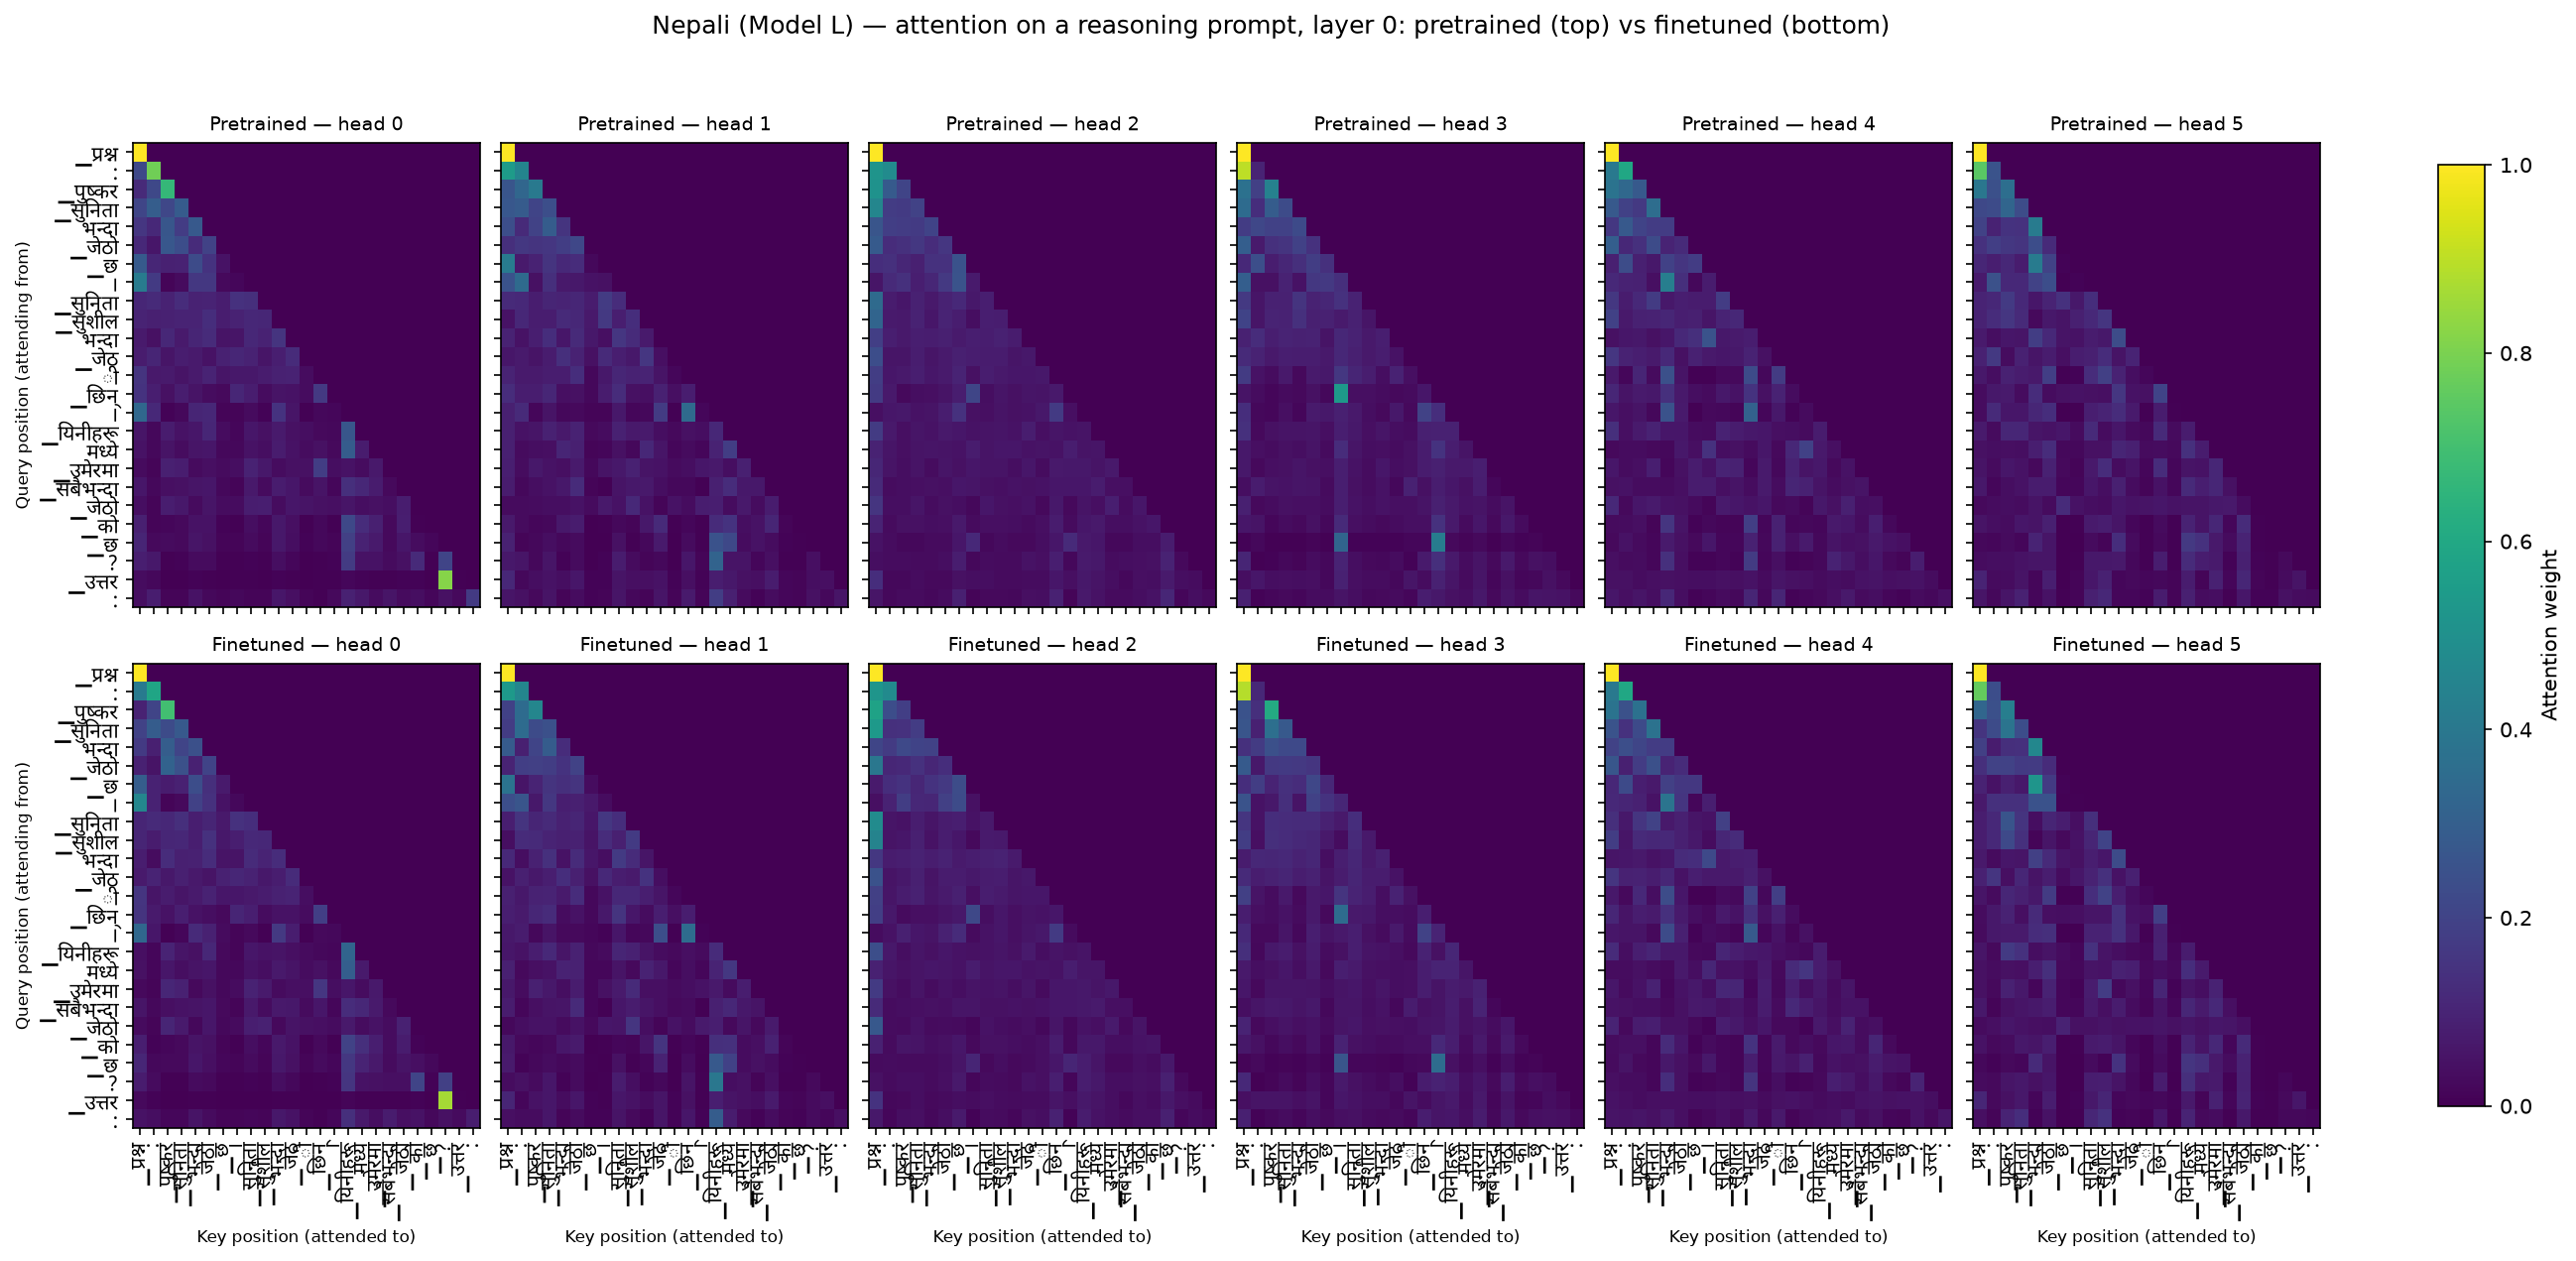
\includegraphics[width=0.495\linewidth]{attention_finetune_nepali_layer0.png}\hfill
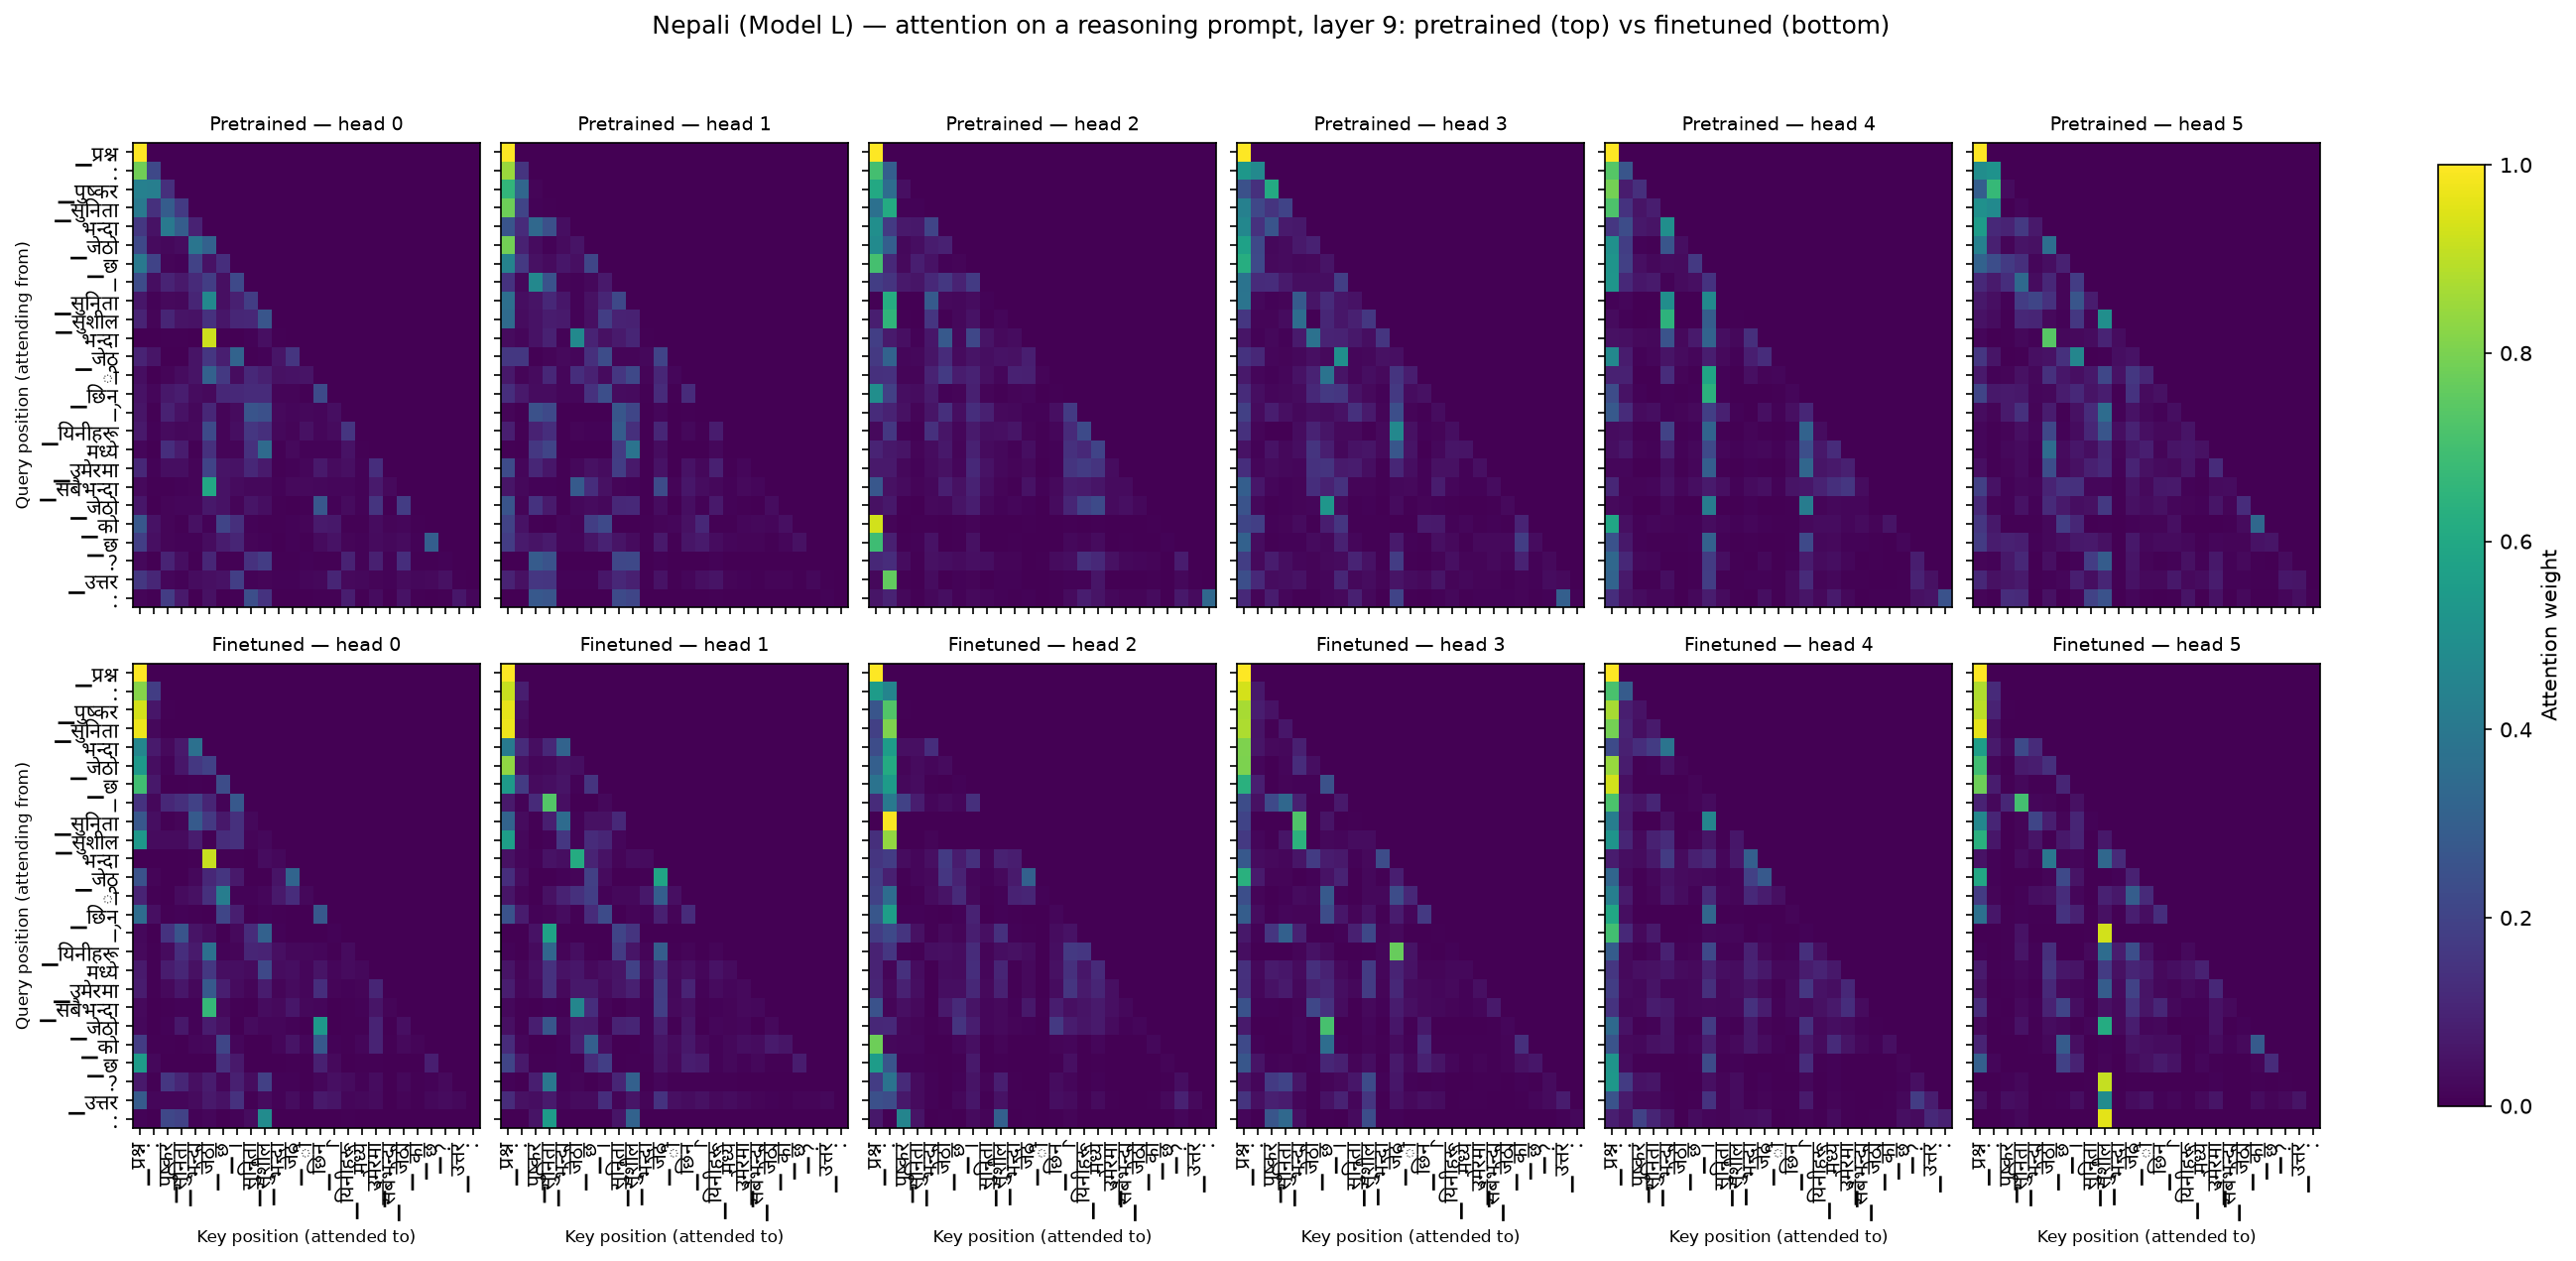
\includegraphics[width=0.495\linewidth]{attention_finetune_nepali_layer9.png}
\caption{Pretrained (top row of each panel) and finetuned (bottom row) attention on one reasoning prompt, for all six heads. Left: layer 0. Right: layer 9. Top: \MH{}. Bottom: \ML{}. Layer 0 is visually unchanged. Table~\ref{tab:attshift} quantifies the late-layer change.}
\label{fig:ftheat}
\end{figure}

\begin{figure}[t]
\centering
\begin{subfigure}[b]{0.54\linewidth}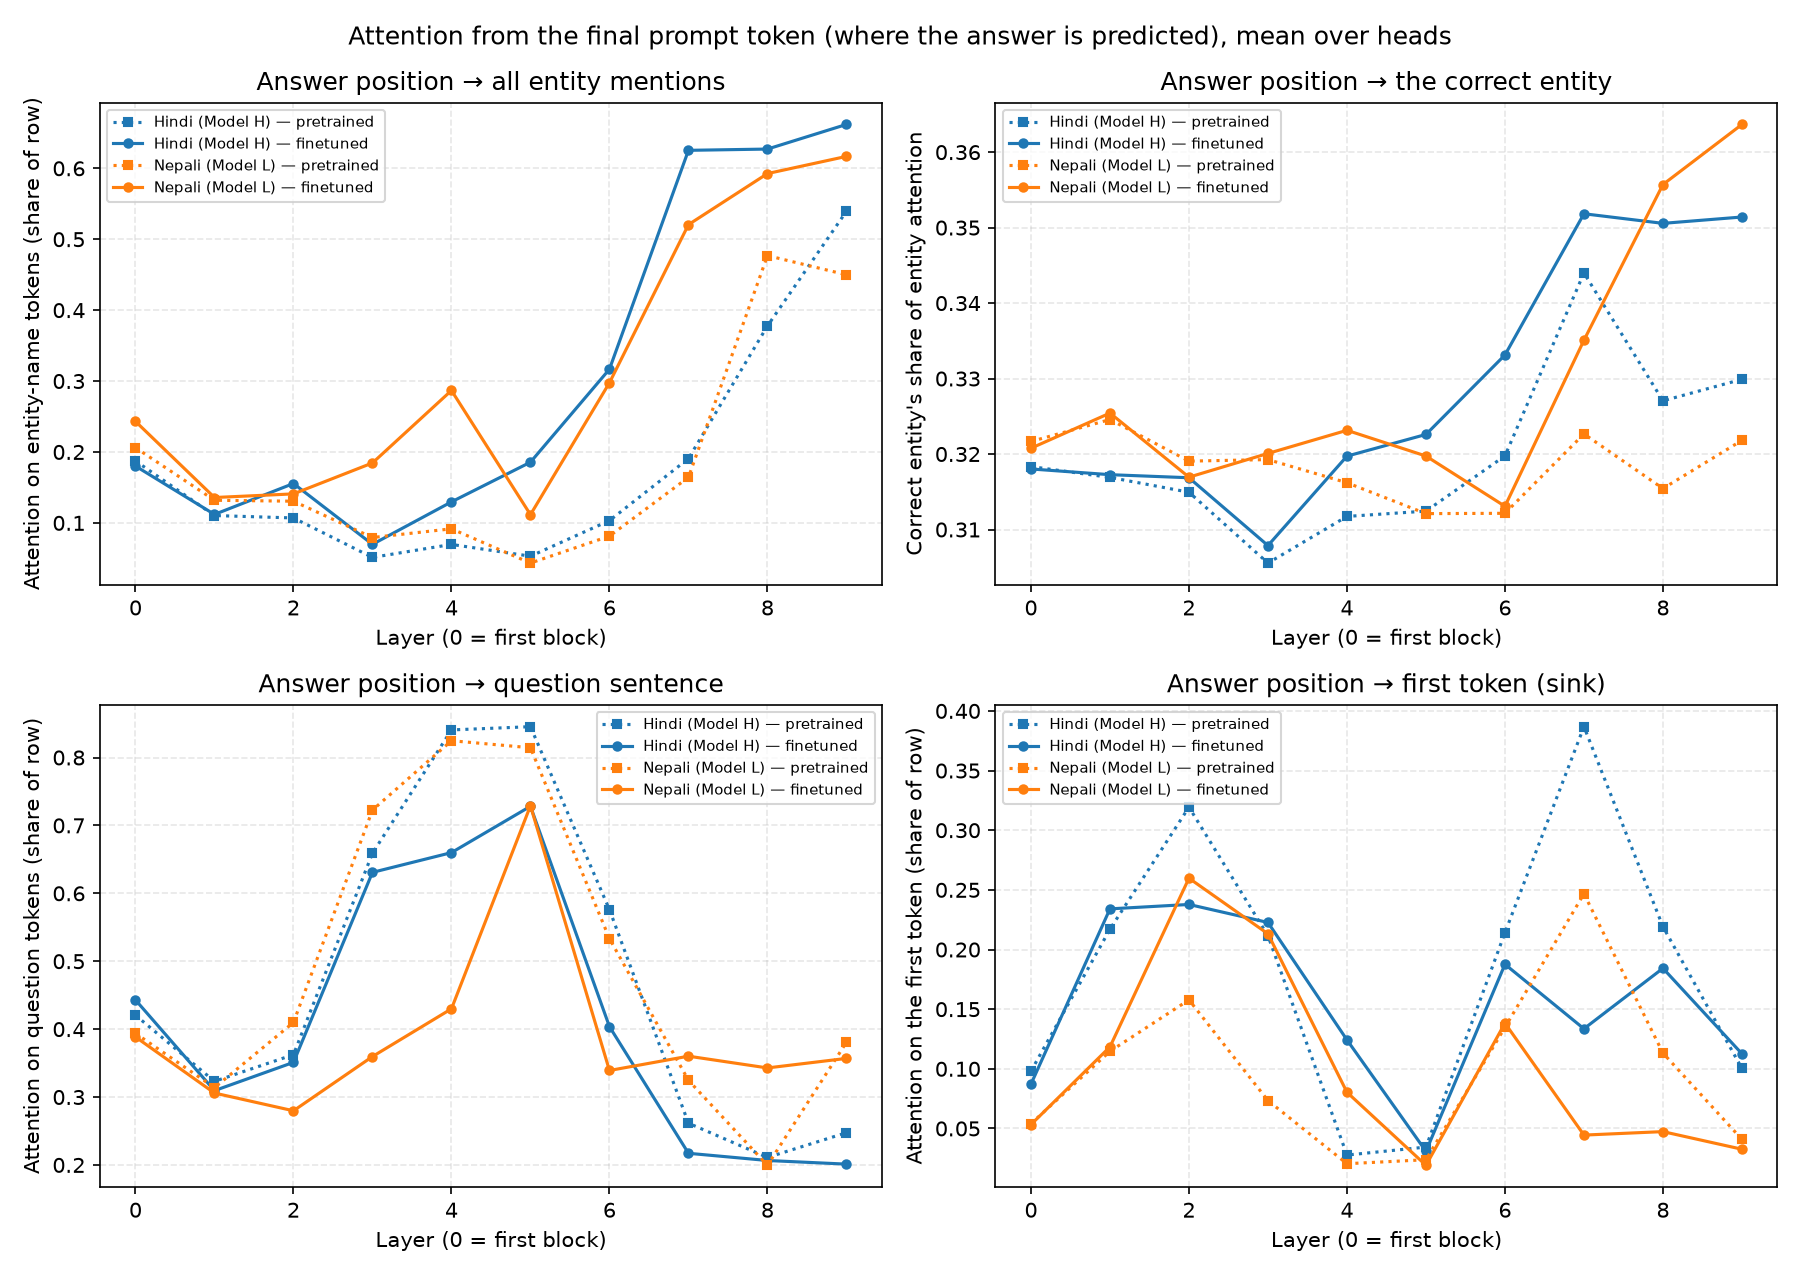
\includegraphics[width=\linewidth]{attention_finetune_answer_position.png}\caption{Where the answer position attends, by layer.}\end{subfigure}\hfill
\begin{subfigure}[b]{0.44\linewidth}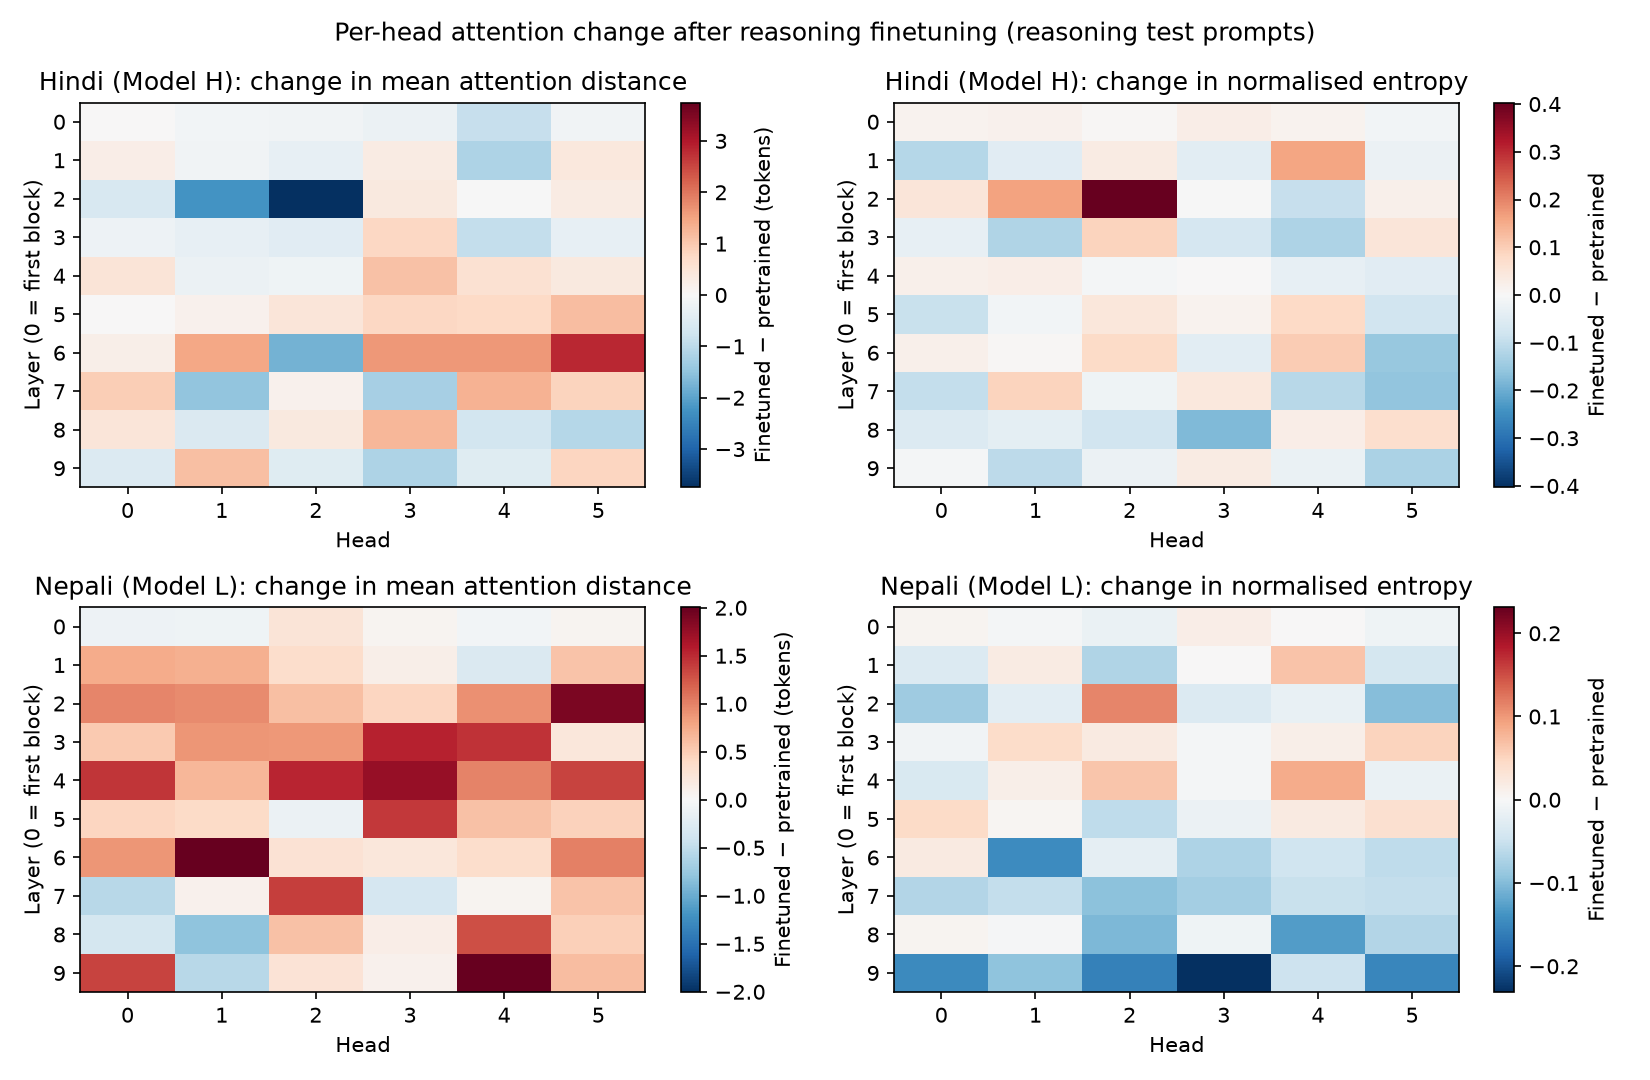
\includegraphics[width=\linewidth]{attention_finetune_head_change.png}\caption{Per-head change (finetuned $-$ pretrained).}\end{subfigure}
\caption{Attention change on reasoning test prompts.}
\label{fig:answerpos}
\end{figure}

\FloatBarrier
% ==========================================================================
\section{Discussion: the four questions}\label{sec:discussion}
% ==========================================================================
\textbf{1. How did data scale and quality differ?}
In tokens, \MH{} had 1.46$\times$ the training data of \ML{} (523.7M against 357.5M). In characters the gap is only 1.21$\times$ (2.02B against 1.67B), because the Nepali tokenizer uses more characters per token.
The quality difference is mostly one of \emph{register}. Before deduplication, Hindi's manual share includes 157k proofread literary documents from Wikisource and 87k Wikipedia articles. Nepali's manual share is mostly news from 18 sites, and news syndication shows up as more near-duplicates (68,243 removed against 59,074, from a similar number of documents).
Nepali also leans more on the downloaded corpora (77.1\% of training tokens against 70.5\%).

\textbf{2. How do language-modelling and reasoning results compare across the tiers?}
Language modelling gives no clean ranking. \MH{} is ahead on perplexity (42.9 against 47.1) and \ML{} on bits-per-byte (0.448 against 0.557), and because each model is scored on its own language's text, neither metric shows that one model knows its language better. The two models' generations share the same failure modes.
Reasoning separates them a little more. \MH{} is 3.0 points above chance on \code{test} and 6.0 points above it on four-hop chains, while \ML{} is at chance on \code{test} and 5.1 points below it on four-hop chains.
The resource gap therefore shows up as a small advantage for \MH{} on reasoning, not as a different kind of model. With one seed per model, that gap should be read as suggestive rather than established.

\textbf{3. Which tokenizer and corpus factors most affected the lower-resource model?}
(i)~\emph{Corpus size, set by the manual floor.} \ML{} had one epoch over 0.71$\times$ the token target, and its validation loss was still falling when the data ran out (3.755$\to$3.741 over its last 30M tokens, although part of that fall comes from the learning rate annealing).
(ii)~\emph{Tokenization, which cuts both ways.} Nepali fertility per word is 6.7\% higher (1.369 against 1.282; Table~\ref{tab:tokenizer}), but that does not mean the tokenizer is worse: Nepali writes postpositions as part of the word (रामको, सुनिताभन्दा), so its words are longer. Per character, Nepali tokens are \emph{coarser} (4.68 against 3.96 characters per token). Each Nepali prediction therefore covers more text, which raises perplexity, lowers bits-per-byte, and leaves fewer tokens from the same amount of text.
(iii)~\emph{Register.} A news-dominated manual share gives less variety of sentence structure than Hindi's literary text.

\textbf{4. What evidence explains the observed differences?}
The perplexity and BPB rankings flip because bytes per token differ by 27\%, which isolates the tokenizer's contribution.
The loss curves (Fig.~\ref{fig:loss}) show \ML{} still improving when its corpus ends.
Attention statistics show \ML{} with fewer specialised heads and less differentiated late layers (10 sharp heads against 16, and a late-layer distance spread of 61 positions against 125), which is consistent with less data buying less specialisation.
In finetuning, \ML{} fell back on the ``both equal'' answer in half of its greater/smaller pair questions and stayed below chance on longer chains, and in both models attention analysis shows the gain came from looking at entities rather than choosing between them.
One caveat applies throughout: loss curves in nats per token are not tokenizer-independent, so only the byte-normalised numbers compare the two languages directly.

% ==========================================================================
\section{Limitations}
% ==========================================================================
Every result is from a single seed. The reasoning accuracies are close enough to chance that seed variance could reorder the two models.
Choice accuracy sums log-probabilities, which penalises multi-token candidates such as ``both equal'' and partly explains the pretrained model's 0\% rate on that answer.
The reasoning task asks for one answer token with no intermediate steps, which is a hard setting for a 24M model. A supervised scratchpad that states the intermediate comparisons would be the natural next experiment.
BLEU, chrF and ROUGE-L use one reference per prompt.
The optional no-positional-embedding ablation was not run.

% ==========================================================================
\section{Reflections}
% ==========================================================================
\todo{This section must be in your own words: the brief grades your reflections. The points below are draft prompts drawn from the project history. Rewrite, cut or replace them.}
\begin{itemize}
\item \textbf{Asserting beats eyeballing.} The bugs that mattered most were silent: splitting heads along time, which still trains; a ROUGE package that scores all Devanagari as zero; deduplication quietly eroding the manual share. Each was caught by a test or a measured statistic, not by a loss curve.
\item \textbf{The model predicts the next token; it does not understand what it says.} Building one from scratch made this concrete for me. At $T{=}1.0$ both models write fluent, grammatical Hindi and Nepali, with correct postpositions, agreeing verbs and a danda at the end, while inventing numbers that contradict each other within a sentence. The reasoning finetune showed the same thing more sharply: the models learned to answer with a name from the prompt, but picked it by shortcuts (the last-mentioned name, a default ``no'' or ``both equal''), and their attention moved towards the entities without favouring the correct one. Nothing in the training objective asks the model to be right, only to make the next token likely, so fluent output is not evidence of understanding.
\item \textbf{A near-chance result is a result.} The first finetune looked like it was learning until held-out names showed it had memorised training names. It would have been easy to keep tuning until validation accuracy looked good. Reporting accuracy against chance, and checking which shortcuts the model uses, told me more.
\item \textbf{What I would do differently:} build the reasoning evaluation and its shortcut checks \emph{before} the first finetune; run at least three seeds; supervise intermediate comparisons; and start manual Nepali collection earlier to lift the token budget.
\end{itemize}

% ==========================================================================
\section{Reproducibility and use of AI tools}
% ==========================================================================
The README gives the full command sequence (steps 1--17) and public Google Drive links for corpora, token arrays, and pretrained and finetuned checkpoints. Run logs (\code{config.json}, \code{metrics.jsonl}, \code{train.log}), evaluation outputs and per-example predictions are committed under \code{<Language>/runs/}.
Every table here is regenerated by \code{python -m common.report.final}, and every figure by the evaluation and figure commands in the README.

\textbf{Use of AI tools.} I used Claude during this project. In my assignment used it mainly as a tutor: to explain concepts such as attention scaling, tokenizer evaluation and checkpoint resumption, and to review and debug my code.

% ==========================================================================
\section*{References}
\vspace{-4pt}
{\footnotesize
\setlength{\columnsep}{14pt}
\begin{multicols}{2}
\renewcommand{\section}[2]{}
\begin{thebibliography}{99}\setlength{\itemsep}{0pt}
\bibitem{vaswani} A.~Vaswani et al. Attention is all you need. \emph{NeurIPS}, 2017.
\bibitem{gpt2} A.~Radford et al. Language models are unsupervised multitask learners. OpenAI, 2019.
\bibitem{prenorm} R.~Xiong et al. On layer normalization in the Transformer architecture. \emph{ICML}, 2020.
\bibitem{tying} O.~Press and L.~Wolf. Using the output embedding to improve language models. \emph{EACL}, 2017.
\bibitem{adamw} I.~Loshchilov and F.~Hutter. Decoupled weight decay regularization. \emph{ICLR}, 2019.
\bibitem{sentencepiece} T.~Kudo and J.~Richardson. SentencePiece: a simple and language independent subword tokenizer and detokenizer. \emph{EMNLP (Demo)}, 2018.
\bibitem{unigram} T.~Kudo. Subword regularization: improving neural network translation models with multiple subword candidates. \emph{ACL}, 2018.
\bibitem{ccnet} G.~Wenzek et al. CCNet: extracting high quality monolingual datasets from web crawl data. \emph{LREC}, 2020.
\bibitem{sangraha} M.~S.~U.~R.~Khan et al. IndicLLMSuite: a blueprint for creating pre-training and fine-tuning datasets for Indian languages. \emph{ACL}, 2024.
\bibitem{bleu} K.~Papineni et al. BLEU: a method for automatic evaluation of machine translation. \emph{ACL}, 2002.
\bibitem{chrf} M.~Popović. chrF: character n-gram F-score for automatic MT evaluation. \emph{WMT}, 2015.
\bibitem{rouge} C.-Y.~Lin. ROUGE: a package for automatic evaluation of summaries. \emph{ACL Workshop}, 2004.
\bibitem{sacrebleu} M.~Post. A call for clarity in reporting BLEU scores. \emph{WMT}, 2018.
\bibitem{degeneration} A.~Holtzman et al. The curious case of neural text degeneration. \emph{ICLR}, 2020.
\bibitem{sinks} G.~Xiao et al. Efficient streaming language models with attention sinks. \emph{ICLR}, 2024.
\end{thebibliography}
\end{multicols}
}

\end{document}
